\label{chap:basics}
This is basics.
	\section{Formal power model}
	\label{sec:power_model}
	
	\section{Heuristics}
	\label{sec:heuristics}
	There are a lot of existing heuristics. At the early time of heuristics usage, the algorithms are applied to solve one
	particular optimization problem. These problem-dependent heuristics cannot be adapted to other optimization processes.
	To improved the portability of heuristics, some algorithms are invented as parameterized interface that can be widely
	deployed for a variety of optimization problems. Such problem-independent heuristics usually consist of a base framework
	with several parameters. Only the parameters are related to the optimization problems. When using one of those
	heuristics for different problem sets, the algorithm framework is common while the parameters should be set up according
	to the problem requirements. In the recent years, there is a new trend of heuristic which is called hyper-heuristic.
	The hyper-heuristics provide a high-level strategy to seek one or several low-level heuristics to generate a proper algorithm for solving an optimization problem. The hyper-heuristic is a cutting-edge technique and it is beyond the knowledge of this work. For the memory power optimization, the problem-independent heuristics are the mainly focused
	because of its extensive usage.
	
	There are a variety ways to classify the heuristics. One common classification is to differentiate the algorithms
	according to their searching mechanisms. To be simplified, the heuristics are divided as local search-based and
	non-local search-based in this work. The well known local search algorithm aims to seek for the optimal solution by
	iteratively moving to a better solution in the neighborhood. However, the local search is greedy and cannot guarantee providing the good enough solutions because it may trap in local optimums. The idea of local search-based heuristics
	is to avoid the local optimum trap through some criteria for solution selection and improve the result's quality.
	Heuristics of this kind output only one single optimal solution. Some classical local search-based heuristics are simulated annealing, tabu search, guided local search, etc. Unlike local search-based heuristics, the non-local search-based heuristics usually seek for a set of good enough solutions. By manipulating some defined solution characteristics, it can guide the searching process to the global optimums. Some typical non-local search-based heuristics are genetic algorithm, particle swarm optimization, ant colony optimization, etc.
	Normally, the frameworks of non-local search-based heuristics are more complicated than that of local search-based algorithms. And the expected result for memory power optimization is one optimal configuration not a set of
	configurations. Therefor, the local search-based heuristics are main focuses in this work.
	In this section, the local search algorithm along with its local optimum trap is discussed first. Then, two typical
	local search-based heuristics, tabu search and simulated annealing, are represented. Lastly, the most promising algorithm 
	is proposed to the memory power optimization according to the comparison between these heuristics.
	
		\subsection{Local search algorithm}
		\label{subsec:local_search}
		Local search algorithm is one of the simplest heuristics. Given a optimization problem, it starts from an initial solution and searches in the current solution's neighborhood. If a better solution is found, the current solution is replaced by it. The searching process is repeated until there is no better solution in the current solution's neighborhood. Then it outputs the current solution as the algorithm result.
		Algorithm \ref{algo:local_search} shows the pseudo-code of local search process. There are four main steps in the algorithm. First step is finding a initial solution and set it as the current solution. The initial solution should be valid for the problem. In the second step, a neighboring solution is generated by certain mechanism. And the third step is to compare the neighboring solution with the current one through a object function. The object function is a method to indicate how good the solution is. The last step is the selection criterion for solution. Local search algorithm selects the better one between the current and neighboring solutions, which is a naive criterion.
		
			\begin{algorithm2e}[H]
				\KwData{an optimization problem}
				\KwResult{an optimal solution}
				current solution = initial solution\;
				\While{not terminate}
				{
					generate a neighboring solution\;
					evaluate the neighboring solution\;
					\If{neighboring solution is better than current solution}
					{
						current solution = neighboring solution\;
					}
				}
				output current solution\;
				\caption{Local Search Algorithm}
				\label{algo:local_search}
			\end{algorithm2e}
		
		Though local search algorithm is simple, the solution it provides may be the local optimal one. This is the major problem of
		local search algorithm. Figure \ref{fig:local_optimum_local_search} illustrates this local optimum trap. Suppose the
		optimization problem is to find the solution with minimum cost, the local search algorithm starts with the initial solution $a$.
		The cost of neighboring solution $b$ is lower than cost of $a$, then $b$ becomes the current solution. The same searching process 
		is repeated until the current solution reaches $c$. There is no better solution in $c$'s neighborhood, thus the algorithm outputs solution $c$ and terminates. However, solution $c$ is only the local optimum and the global optimum is solution $e$ which
		is not in $c$'s neighborhood. In order to reach solution $e$, the algorithm has to move to solution $d$ whose cost is higher than
		$c$'s cost. And this violates the selection criterion of the algorithm. Another drawback of local search algorithm is that the result quality is dependent on the initial solution. If the algorithm starts with solution $d$, the output will be the global optimum $e$. These two disadvantages make local search algorithm an improper choice when global optimal solution is required for 
		the optimization problems.
		
			\begin{figure}[H]
				\begin{center}
					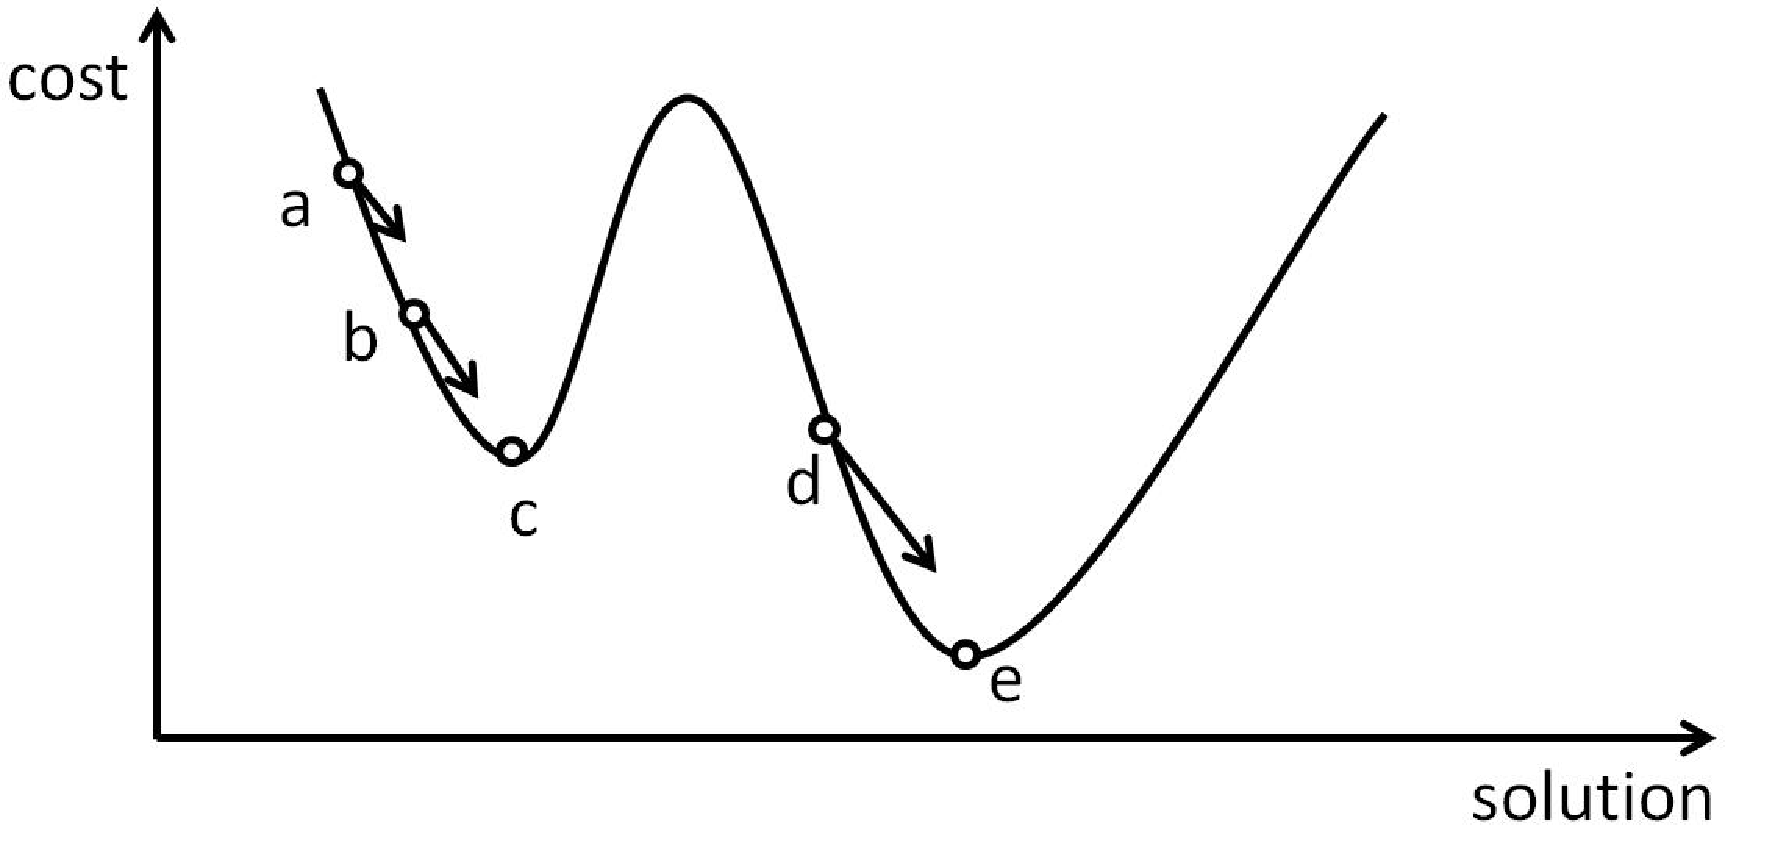
\includegraphics[width=0.7\textwidth]{local_optimum_local_search}
					\caption[Local Optimum Problem]{Local Optimum Trap}
					\label{fig:local_optimum_local_search}
				\end{center}
			\end{figure}
		
		\subsection{Tabu search algorithm}
		\label{subsec:tabu_search}
		One of the improvements to local search is the tabu search algorithm. It is based on local search but it avoids to stuck at the
		local optimal trap through a different selection criterion for solutions. As discussed in section \ref{subsec:local_search}, once
		the local search algorithm is trapped at a local optimal solution, it cannot move any further due to the naive solution criterion.
		
		
		
		
		
		
		
		
		
		
		
		
		